\chapter{Диаграмма прецедентов}

\begin{figure}[h]
    \centering
    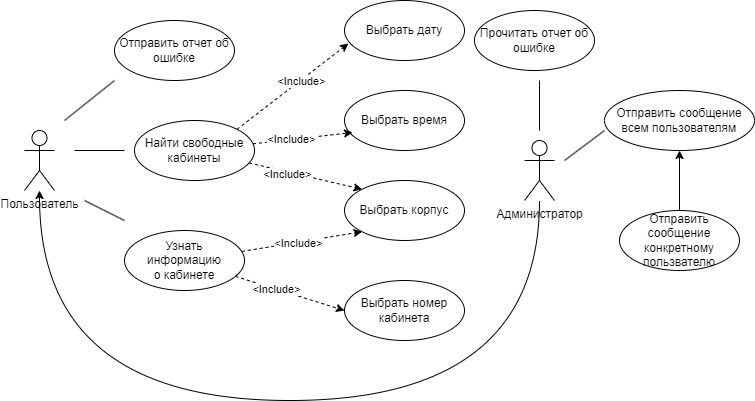
\includegraphics[scale=0.6]{img/prec}
    \caption{Диаграмма прецедентов}
    \label{fig:cp}
\end{figure}

Актеры:

Пользователь: Основной пользователь системы. Его действия в системе направлены
на получение информации о кабинетах.
Администратор: Ответственный за управление системой. Его функции включают в себя
прочтение отчетов об ошибках и отправку сообщений пользователям.

Прецеденты Пользователя:

Узнать информацию о кабинете: Пользователь может запросить информацию о
конкретном кабинете. Для этого ему потребуются следующие дополнительные
действия:

Выбрать корпус: Пользователь выбирает интересующий его корпус.

Выбрать номер кабинета: После выбора корпуса, пользователь указывает номер
интересующего его кабинета.

Аналогично пользователь может получить список свободных кабинетов, введя дату и
время.

Отправить отчет об ошибке: Если пользователь обнаружил ошибку в информации или в
работе системы, он может отправить отчет администратору.

Прецеденты Администратора:

Прочитать отчет об ошибке: Администратор имеет возможность просмотреть
полученные отчеты об ошибках от пользователей.

Отправить сообщение всем пользователям: В случае необходимости администратор
может отправить сообщение всем пользователям системы.

Отправить сообщение конкретному пользователю: Администратор может направить
сообщение определенному пользователю, например, чтобы уточнить детали отчета об
ошибке или предоставить индивидуальную информацию.

Отношения между прецедентами:
Администратор может выполнять все функции, доступные пользователю.

\chapter{Карта сайта}

\begin{figure}[h]
    \centering
    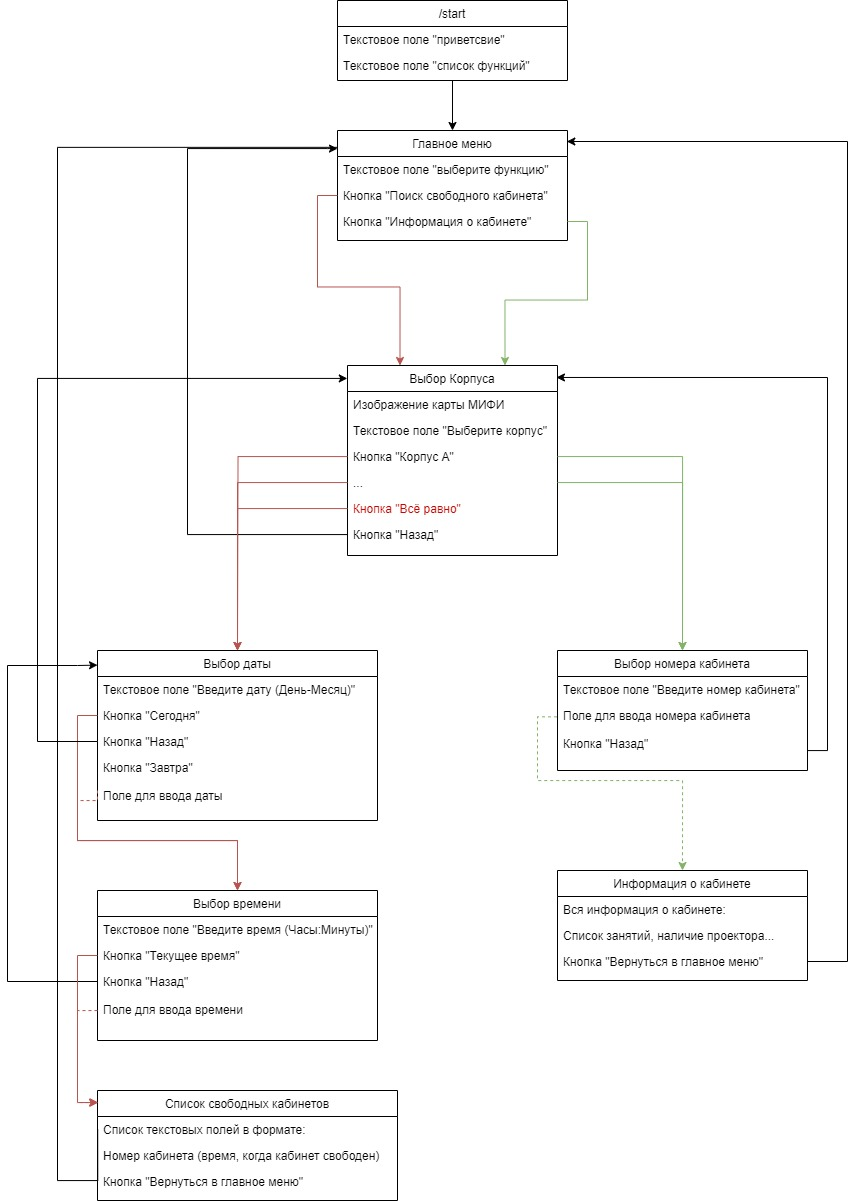
\includegraphics[scale=0.45]{img/map}
    \caption{Карта сайта}
    \label{fig:cp}
\end{figure}

1. Стартовое меню:

При запуске бота пользователь видит приветственное сообщение и список доступных
функций:

Поиск свободного кабинета

Информация о кабинете

Пользователь может выбрать одну из предложенных функций, нажав соответствующую
кнопку.

2. Выбор корпуса:

При выборе поиска свободного кабинета пользователь должен указать корпус здания,
в котором будет произведен
поиск (существует опция поиска по всем корпусам) либо вернуться в главное меню.
Для удобства пользователя бот покажет карту университета.

3. Выбор даты:

Пользователь вводит дату в формате (День-Месяц), либо может вернуться на
предыдущий этап.

Для удобства пользователя всплывают кнопки:
"Сегодня": При выборе этой кнопки поиск будет проводиться на текущую дату.
"Завтра": При выборе этой кнопки поиск будет проводиться на следующий день.

4. Выбор времени:

После выбора даты пользователь указывает время в формате (Часы:Минуты), либо
может вернуться на предыдущий этап.

Для удобства пользователя всплывает кнопка:
"Текущее время": При выборе этой кнопки поиск будет проводиться на текущее
время.

5. Список свободных кабинетов:

После ввода всех параметров пользователю выводится список свободных кабинетов:

Список текстовых полей: Каждое поле содержит информацию о свободном кабинете
(номер кабинета, интервал времени, когда кабинет освободится).
Также появится кнопка "Вернуться в главное меню".

6. Выбор номера кабинета:

Если пользователь хочет узнать информацию о конкретном кабинете, то после выбора
корпуса
ему необходимо ввести номер желаемого кабинета.

7. Информация о кабинете:

Вся информация о кабинете: Список занятий, наличие проектора и др.
Также появится кнопка "Вернуться в главное меню": Возврат в главное меню.

\chapter{Схема базы данных}

Данная система должна хранить в себе следующие данные:
\begin{itemize}
    \item Информацию о аудиториях в НИЯУ МИФИ, включая их характеристики, такие
как наличие проектора, компьютера...
    \item Данные о пользователях системы.
    \item Подробности о занятиях, такие как их тип, предмет, время начала и
окончания, дни проведения, семестр и аудитория.
    \item Информацию о преподавателях, включая их короткие имена или инициалы.
    \item Сведения о студенческих группах.
\end{itemize}

Можно заметить, что данные, которые необходимо хранить, обладают четкой
структурой и имеют связи. Например, каждый урок связан с конкретной аудиторией и
может быть связан с несколькими преподавателями или студенческими группами. Эти
связи помогут в организации расписания и оптимизации использования ресурсов
учебного заведения.

Важными факторами при выборе системы управления базы данных являются:
\begin{itemize}
    \item Производительность: Система должна быстро обрабатывать запросы и
обеспечивать минимальные задержки при работе с большим объемом данных.
    \item Масштабируемость: Возможность расширения системы для работы с
увеличивающимся объемом данных без значительного снижения производительности.
    \item Надежность: Гарантия сохранности данных даже при возникновении
технических сбоев.
    \item Безопасность: Защита данных от несанкционированного доступа и утечек.
    \item Поддержка: Наличие обширной документации, сообщества пользователей и
профессиональной технической поддержки.
\end{itemize}

\begin{figure}[h]
    \centering
    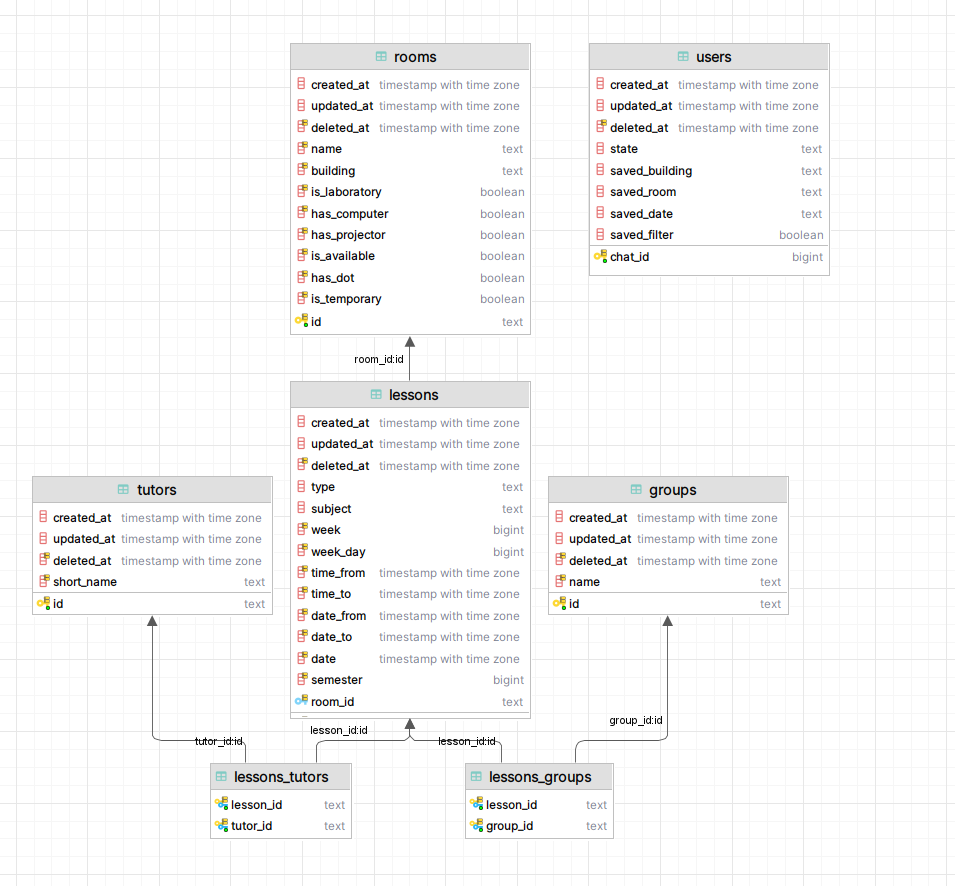
\includegraphics[scale=0.6]{img/bd}
    \caption{Схема базы данных}
    \label{fig:cp}
\end{figure}


\subsection*{1. Таблица ``rooms'' (Кабинеты):}
Эта таблица содержит информацию о аудиториях в НИЯУ МИФИ.
\begin{itemize}
    \item \textbf{created\_at, updated\_at, deleted\_at}: Даты создания,
обновления и удаления записи.
    \item \textbf{name}: Название аудитории.
    \item \textbf{building}: Здание, в котором находится аудитория.
    \item \textbf{is\_laboratory}: Флаг, указывающий, является ли аудитория
лабораторией.
    \item \textbf{has\_computer, has\_projector}: Флаги, указывающие на наличие
компьютера и проектора в аудитории.
    \item \textbf{is\_available}: Доступность аудитории.
    \item \textbf{has\_dot, is\_temporary}: Дополнительные характеристики
аудитории (ДОТ, выездная аудитория).
    \item \textbf{id}: Уникальный идентификатор аудитории.
\end{itemize}

\subsection*{2. Таблица ``users'' (Пользователи):}
Содержит информацию о пользователях системы.
\begin{itemize}
    \item \textbf{created\_at, updated\_at, deleted\_at}: Даты создания,
обновления и удаления записи.
    \item \textbf{state}: Состояние пользователя.
    \item \textbf{saved\_building, saved\_room, saved\_date}: Сохраненный запрос
пользователя (здание, комната и дата).
    \item \textbf{saved\_filter}: Сохраненный запрос пользователя (наличие
проектора в аудитории).
    \item \textbf{chatId}: Идентификатор чата пользователя в Telegram.
\end{itemize}

\subsection*{3. Таблица ``lessons'' (Уроки):}
Информация о уроках или занятиях.
\begin{itemize}
    \item \textbf{created\_at, updated\_at, deleted\_at}: Даты создания,
обновления и удаления записи.
    \item \textbf{type, subject}: Тип(Лек, Пр...) и название предмета.
    \item \textbf{week, week\_day}: Неделя и день недели пары.
    \item \textbf{time\_from, time\_to}: Время начала и окончания пары.
    \item \textbf{date\_from, date\_to}: Даты начала и окончания пары.
    \item \textbf{semester}: Семестр.
    \item \textbf{room\_id}: Идентификатор комнаты, в которой проводится урок.
\end{itemize}

\subsection*{4. Таблица ``tutors'' (Преподаватели):}
Информация о преподавателях.
\begin{itemize}
    \item \textbf{created\_at, updated\_at, deleted\_at}: Даты создания,
обновления и удаления записи.
    \item \textbf{short\_name}: Инициалы преподавателя.
    \item \textbf{id}: Уникальный идентификатор преподавателя.
\end{itemize}

\subsection*{5. Таблица ``groups'' (Группы):}
Содержит информацию о студенческих группах.
\begin{itemize}
    \item \textbf{created\_at, updated\_at, deleted\_at}: Даты создания,
обновления и удаления записи.
    \item \textbf{name}: Название группы.
    \item \textbf{id}: Уникальный идентификатор группы.
\end{itemize}

\subsection*{6. Таблица ``lessons\_tutors'' (Пары и преподаватели):}
Связывает пары с преподавателями.
\begin{itemize}
    \item \textbf{lesson\_id, tutor\_id}: Идентификаторы урока и преподавателя.
\end{itemize}

\subsection*{7. Таблица ``lessons\_groups'' (Пары и группы):}
Связывает пары со студенческими группами.
\begin{itemize}
    \item \textbf{lesson\_id, group\_id}: Идентификаторы урока и группы.
\end{itemize}